\chapter{Validation of Aggregators Providing Demand Response}\label{app:pscc2016}

\textbf{Authors:}\\
Daniel Esteban Morales Bondy\\
Oliver Gehrke\\
Anders Thavlov\\
Kai Heussen\\
Anna M. Kosek\\
Henrik W. Bindner

\noindent
\textbf{Submitted to:}\\
Power Systems Computational Conference, 2016 \\
Genoa, Italy


\noindent
\textbf{Abstract:}\\
As aggregators become viable sources of ancillary services, they will be required to undergo a validation process similar to the prequalification process of traditional generators. Since aggregators are fundamentally different from traditional generators, a new test method must be designed for the aggregator validation. This work proposes a method for designing the tests necessary for the validation process. The method is exemplified with a study case and results are presented.

\section{Introduction}
As renewable energy generation increasingly replaces conventional power plants, power system operators are looking for alternative sources for the ancillary services which were traditionally provided by these plants. It is expected that some ancillary services can be procured from distributed consumption and production units by making use of their unused operational flexibility. In order to provide coordinated services, such as demand response \cite{macdonald2012demand}, from a large number of such distributed energy resources (DERs), a new actor is appearing in the power system: the aggregator \cite{gkatzikis2013a}.% \hl{I was wondering whether we should clarify which type of aggregator we're talking about here, to make it harder for nitpicking reviewers.}\textcolor{red}{You mean commercial VPP vs Technical VPP?}

Conventional sources for ancillary services must be certified before being able to offer control reserves in an ancillary services market \cite{energinet2012ancillary}. It is expected that aggregators will be required to undergo a similar prequalification process to ensure the appropriate performance of the provided service with respect to predefined requirements.

The achievable performance of aggregators, in terms of service provision, depends on its architecture \cite{bondy2015a}, i.e. where the decision making is located \cite{kosek2013overview} and its level of automation, the choice of hardware for implementation, the specification of communication protocols \cite{kiliccote2010open}, how advanced the portfolio management is, etc. This means that some aggregator architectures will be better suited for a specific ancillary service than others \cite{bondy2014performance}. 

It has been established that current requirements for participation in the ancillary services markets limit the participation of aggregators of demand response \cite{cappers2013assessment,coalition2014mapping}. Different research projects have looked into this problem, see e.g. \cite{bondy2014flech}. 

Until now, the performance evaluation and testing of aggregators in academia has been ad-hoc to specific aggregator implementations \cite{vrettos2015integrating,rahnama2014evaluation}. Aggregator test frameworks have been proposed \cite{buscher2015towards}, field tests have been carried out in order to validate DR schemes \cite{kiliccote2013field}, and concepts regarding systematized testing have been exemplified \cite{steinbrink2015challenges}.

This work addresses the gap between all these concepts, i.e. we present a procedure for the design of validation tests, which takes a systematical approach to aggregator testing, discussing the issue from input, i.e. service requirements, to output, i.e. performance metrics.

%This work addresses the gap between all these concepts, i.e. the design of a test procedure that takes a systematical approach to aggregator testing, discussing the issue from input, i.e. service requirements, to output, i.e. performance metrics.

%Therefore new methods and tools are needed to validate an aggregator architecture, in terms of capability to deliver the desired services. %Such an assessment of an aggregator can be relevant before investments into a particular infrastructure are made. The methods may also be incorporated into an aggregator prequalification process.

%The purpose of this paper is to derive the testing specification for an aggregator from its contracted service requirements. Specifically, we constrain the analysis to active power services such as frequency containment and frequency restoration reserves \cite{entso1operational} for transmission systems and congestion management for distribution systems. The novelty presented in this work is a method for designing validation tests for aggregators. \hl{How can I give this more oomph?!}

%of the interaction between the systems interacting directly or indirectly with the aggregator. \textcolor{red}{The word interaction is used too much here, how do I fix this?}\hl{I'm not sure if I know what you want to say. "testing of the interaction between the systems interacting with the aggregator" - what interacts with what here? My best bet right now is "The purpose of this paper is to describe the alignment of service requirements with the testing specification of the aggregator, including the interaction between its subsystems." Is that what you meant?}


\section{Conventional resource validation and aggregator differences}\label{sec:PSSCCconventionalvalidation}
%\hl{ We explain why system operators want resources to be validated (WHY?) }
Ancillary services are essential for the reliability of the power system. Because these services play such an important role in the safe operation of the system, it is important that the units or entities providing a service perform according to the requirements set by the Transmission System Operator (TSO). These requirements and processes are typically specific to a particular TSO and influenced by national regulations, interconnection grid codes etc. We will discuss two examples below:

In Denmark, energinet.dk, the Danish TSO, ensures this by requiring all units participating in the ancillary service markets to provide a documentation of their capabilities and go through an approval process \cite{energinettender}. This approval process consists of a test conducted at least three weeks prior to the service delivery date. The tests for Frequency Containment Reserve generally involves the injection of a setpoint step into the plant's governor and the measurement of the response. The test for Automatic Frequency Restoration Reserve involves the tracking of a reference signal from energinet.dk. Currently, this procedures are not formally described.
Demand resources are expected to provide a substantial amount of the ancillary services for the Danish grid in the future. Since distribution system services are not widespread yet, the concept of unit certification is non-existent at the distribution level. 

%\hl{Here we explain the current method for resource validation. (HOW?)}
%\hl{There is abig jump form Demnark to US, maybe we can sat that Denmark has not such regulations and US is more advanced in the process...}
While Denmark is starting to open up to new sources of ancillary services and standardise its test procedures, PJM (a regional transmission operator in the United States) has a standardised prequalification procedure for regulating resources\footnote{Regulation in the US corresponds roughly to frequency restoration reserves of ENTSO-E.}, which consists of three consecutive area regulation tests, where PJM Performance Compliance scores indicate how well the resource follows a simulated regulation signal. A single test lasts for 40 minutes and in order to pass it the unit must score at least 75\% in three consecutive tests \cite{pjm2015balance}. While this rule includes services provided by multiple generators at a single site, operators of demand resources are not required to be certified but must complete an initial training module on the requirements and business rules of the Regulation and Synchronized Reserve markets \cite{pjm2015certification}. Currently demand resources are only allowed to form 25\% of the total regulation \cite{pjm2015ancillary} in PJM, and therefore their certification process is still not a large concern. 

In both systems the validation tests have two goals: to ensure the communication with the units works correctly, and to validate the known performance model of the generators. Thus, a change of configuration in the setup requires a new certification of the generator.
%\hl{We show in which way the current method is not applicable to aggregators and other distributed / multi-resource service providers, and conclude that an alternative method is needed (WHAT?, problem statement)}

The current tests outlined above are specific to system operators (here, e.g. Energinet.dk and PJM), but follow similar paradigms. 
The conventional test processes outlined above cannot be directly applied to portfolios of aggregated resources, mainly because a common assumption in the process is that the service delivery is performed by a single or small number of units. This allows inference of the unit's ramping capabilities through a response test, based on a known model. 

An aggregator and the portfolio of units under its control behave fundamentally different from large generation units:
\begin{enumerate}
\item Individual generator units are well understood and models describing their static and dynamic properties are readily available. This is not the case for portfolios of aggregated units which are typically heterogeneous and can only be modelled through their statistical properties. This is aggravated by the fact that unit portfolios may be dynamically reconfigured during operation.
\item There might not be a meaningful equivalent to a single point of measurement: An aggregator's portfolio may consist of geographically dispersed units. Their aggregate power profile does not correspond to a measurement at any single point of the grid.
\item Aggregators, by definition, operate a distributed system (both in control and geographical terms) in which each unit has its own response properties and requirements. This leads to an aggregated response that behaves differently from that of conventional generators.
\item Reliability concepts for distributed systems are different; specifically, the failure modes are not the same. If a component of a monolithic generator unit fails, the whole unit may have to shut down. The failure of a single unit in an aggregator portfolio will often have a minor or negligible impact on the overall performance. In a large portfolio it will usually be possible to recruit an equivalent replacement unit providing the same services as the failed one.
%\item There are many different ICT and control architectures for aggregators, and interoperability standards must be used for the internal workings of the aggregator. \hl{and whats the point?}
%\item The primary purpose of units composing an aggregator is to serve a specific energy-dependent need of the unit owner, not to provide the flexibility service, hence not all units in an aggregator portfolio may always be available.\hl{This is a property of e.g. demand response, not of aggregation. It applies to a single DR unit as well. I'd skip this argument.}
\end{enumerate}

For the above reasons, validation cannot be performed on the individual units in an aggregator's portfolio, but has to be applied to the aggregator's control process and portfolio. This paper focuses on the alignment between service requirements and the design of the tests needed for the validation of aggregators. 

%is not as straightforward for aggregated systems due to their geographical distribution, dynamic nature, complex ownership structure, and possible difference between the service requirements of individual units and the aggregate as a whole.
%The service requirements may also differ between demand response and traditional ancillary services, which leads to different validation requirements.\textcolor{red}{better?}

\section{Requirements and proposed test  procedure}\label{sec:metrics}
%\hl{- What alternative method do we propose?}

The objective of the current tests is to validate the parameters of a well understood model of generation units. For the reasons stated previously, the new tests need to identify an empirical behavior model of an uncertain and diverse entity: the aggregator control architecture and unit portfolio. 

%This means that there is no single standard test, but 
A test procedure is required that will allow the system operators to understand and predict the performance of a specific aggregator under a given set of operation conditions (Fig.~\ref{fig:framework}). In this section we present the underlying assumptions for such a procedure, the metrics used to measure the aggregator performance, and the proposed procedure.
%Getting an empirical model of an unknown entity rather than a mathematical model of a known entity. System identification approach.

\begin{figure}[!t]
\centering
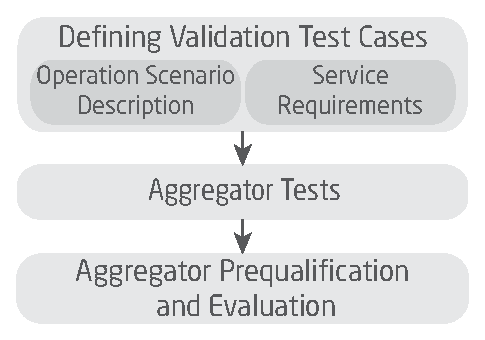
\includegraphics[width=1.7in]{graphics/pscc2016/validation.eps}
\caption{Schematic procedure for aggregator validation. The focus of this paper is on the relationship between the service requirements and the aggregator tests.}
\label{fig:framework}
\end{figure}

%Here the following three topics must be discussed:
%\begin{itemize}
%\item Boundary conditions (grid, DER)
%\item Fault scenarios
%\item Operation spectrum (what is the possibility/range of the input data?)
%\item Experimental design
%\end{itemize}

%The experiments should be able to measure response/states that can't be measured safely/easily under deployment.

%The tests must have a well defined input and output.

\subsection{Test Procedure Assumptions}\label{subsec:assumptions}
%A great variety of aggregator architectures has been proposed and implemented; differences between them are linked to specific business cases, local regulations, grid codes etc. Implementation details such as algorithms for portfolio composition, resource prediction or trading, constitute key intellectual property of commercially operating aggregators and disclosure of these business secrets will be unacceptable in many cases. For this reason,
The critical assumption are:

1) A general test design must start from the assumption that the aggregator and its infrastructure are to be treated as a black box, in the sense that only the aggregator inputs and outputs are known but the details of the internal control architecture are unknown.

%Field tests have been carried out in order to validate DR schemes, see e.g. \cite{kiliccote2013field}. While these kind of tests are important to characterize the capabilities of aggregators, the tests are not able to fully identify their operation capabilities. Thus, i
2) In order to fully test aggregators under a number of relevant scenarios, and to capture the stochastic nature of their operation, aggregators must be tested with the aid of a simulation framework. % While these kind of tests are important to characterize the capabilities of aggregators, the tests are not able to fully identify their operation capabilities.

3) It is assumed that such a simulation framework is detailed enough in terms of power system models, DER models and information and communication technology (ICT) systems in order for the simulation results to reflect the real performance of a deployed aggregator with sufficient precision.
%While a few tests are enough to ensure compliance of traditional generators, the stochastic nature of aggregators requires sufficient samples in order to capture the variance of the stochastic process that influences the aggregator performance. It is usually infeasible to subject a deployed and operational aggregator to a high number of tests, it is expected that aggregator validation must include simulation. In this way, the aggregator will be subjected to situations that are reproducible. 

The assumptions that can be adjusted are:

4) The tests are defined by a set of operational scenarios and service requirements (Fig.~\ref{fig:framework}): a) the operational scenarios define the statistical distribution of the test disturbances; b) the service requirements define the expected behavior of the aggregator. 

5) The mode of interaction between the test cases and the aggregator is defined in a test setup (Fig.~\ref{fig:test_setup}), where the disturbances (test inputs) defined in the operational scenarios affect the aggregator interaction with the DERs and the power grid. 

6) The aggregator has two interfaces: \emph{inputs} in the form of measurements and service reference signals received from the system operators; \emph{outputs} in the form of control domain signals exchanged between the aggregator and the units in its portfolio.

7) The operational scenarios are not designed to cover aggregator operation under exceptional system conditions. This means that the aggregator will not be held accountable for non-delivery in cases where the cause is outside of the aggregator's influence, e.g. in the case of grid faults. If communication between the aggregator and the controlled units, or internally within the aggregator architecture, occurs over public telecommunication networks, the robustness to network outages must be tested, for example by simulating disturbances and delays.

8) The flexibility which the aggregator can offer is bounded by the contractual requirements between the aggregator and its clients.

9) Aggregator validation will be carried out by a third party test entity.

\begin{figure}[!t]
\centering
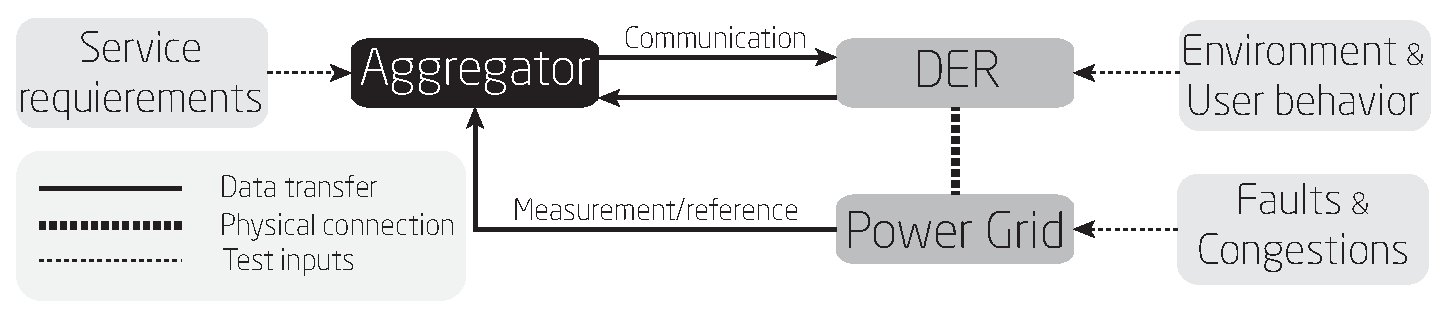
\includegraphics[width=\columnwidth]{graphics/pscc2016/test_setup.eps}
\caption{Schematic test setup where the test subject, the aggregator, is treated as a black box.}
\label{fig:test_setup}
\end{figure}

\subsection{Service Requirements - Test Metrics}\label{sec:servreqmet}

In order to measure how the disturbances affect service delivery, a set of service performance metrics must be established. The main purpose of the current tests is to verify communication, responsiveness to frequency changes and tracking of a reference or AGC\footnote{Automatic Generation Control, see e.g.\cite{entso1operational}.} signal. Coupling this with the performance requirements defined by the TSOs (e.g. \cite{energinet2012ancillary,ipower2013development}), the expected behavior of the considered services was analyzed (Table~\ref{tab:servmet}), and a set of requirement metrics were defined:
\begin{itemize}
\item Time responsiveness, i.e. how fast can the service be delivered from the moment the reference or measurement signal changes.
\item Grid responsiveness, i.e. how well can the aggregator follow changes in the grid state (marked with $\star$ where relevant on Tab.~\ref{tab:servmet}).
\item Response accuracy, i.e. how good is the aggregator in providing the full volume that is requested.
\end{itemize}


\begin{table}[!t]%% increase table row spacing, adjust to taste
\renewcommand{\arraystretch}{1.30}
% if using array.sty, it might be a good idea to tweak the value of
% \extrarowheight as needed to properly center the text within the cells
\caption{System services and their behavior}
\label{tab:servmet}
\centering
% Some packages, such as MDW tools, offer better commands for making tables
% than the plain LaTeX2e tabular which is used here.
\begin{tabularx}{\columnwidth}{p{1.0cm} X X}
\toprule
System Operator& Service name & Service behavior\\
\midrule
TSO & Frequency containment reserve (FCR) & autonomous response to frequency deviations ($\star$) \\
TSO & Frequency restoration reserve (FRR) & tracking of the AGC-signal\\
DSO & Congestion management         & reference tracking \\
    &                               & respecting a maximum feeder/transformer limit ($\star$) \\
    &                               & demand response \\
    &                               & grid state responsiveness ($\star$)\\
\bottomrule
\end{tabularx}
\end{table}

These three metrics will constitute the measure with which an aggregator will be deemed to perform according to service requirements, and the tests must excite the aggregator such that it is possible to determine through the value of these metrics the performance of the aggregator. It must be pointed out that the grid responsiveness metric is only applicable to the evaluation of aggregators providing services that rely on direct measurement of the grid, e.g. FCR.

When system operators define the acceptable values of the service requirement metrics, the values should have a statistical component. An example could be that the time responsiveness of a service provision should in average of 5 seconds, with a variance of $\pm$ 1 second. The actual indices used for the proposed metrics are discussed in Sec.\ref{sec:evaluation}.

\subsection{Aggregator Validation Procedure}\label{sec:alignment}
The procedure for aggregator validation applies statistical principles for the evaluation of the aggregator performance. It consists of the following steps:
\begin{enumerate}
	\item The general composition of the aggregator is established through documentation, and the service the aggregator is to be validated for is selected. %The aggregator informs of the general composition of its portfolio, as well as the service it wants to be validated for.
	\item The testing entity identifies the appropriate service requirements for the selected service.
	\item The testing entity identifies the expected normal operation of the aggregator based upon the service definition.
	\item The testing entity defines the operation scenarios that the aggregator is expected to perform under. %The scenarios must define the statistical properties, e.g. mean and variance, for the stochastic disturbances affecting the aggregator performance.
	\item The tests are carried out on the aggregator.
	\item The aggregator performance is evaluated.
\end{enumerate}

From the services analysed in this work, the tests are divided into two categories depending on their excitation signal:
\begin{itemize}
\item step response (like those for FCR),
\item continuous reference tracking (like those for FRR).
\end{itemize}

The validation tests will use one of these excitation signals under a different set of circumstances defined in the operation scenarios. Sufficient sampling of the aggregator response to the excitation signal is important in order to ensure that the mean and variance of the performance metrics give a realistic impression of the aggregator performance under deployment.%Thus, we formulate the following heuristic for the alignment of service requirements and tests: if a service
%The tests will evaluate the sensitivity of the aggregator to changes in the portfolio, and issues with the communication.


%\hl{The test procedure should be described. 2 diagrams are needed: 1st. shows the aggregator under normal operation (physical connection and the ICT connection), with relevant inputs and outputs of the aggregator. 2nd is the test process, where at each stage inputs are added/modified.}

% At the same time, based upon these two inputs, the overall service delivery is verified and evaluated, which is reflected in the bottom box of Figure~\ref{fig:framework}. \hl{Generally, I think we're still talking too much about the overall process and not about what the paper claims it's focusing on ("[...] the alignment of service requirements with the testing [...]"). On the latter we're not specific enough wrt what kind of result the reader can expect.}

%An aggregator infrastructure and control process is usually complex and therefore interactions of an aggregator may be tested separately. Depending on the metrics by which the relations are measured (Table~\ref{tab:metrics}), it is possible to test certain components through simulation or co-simulation, while other interactions require hardware-in-the-loop tests. This paper will propose a method for identifying the relationships between metric types and the tests necessary  for validating the measured function. The method will then be applied to several existing aggregator architectures as a proof of concept.

\subsection{Evaluation of Test Results}\label{sec:evaluation}
The service requirement metrics (Sec.~\ref{sec:servreqmet}) define the measure upon which the aggregator is evaluated. Different options exist that can be used to measure these metrics. One option is the aggregator performance index \cite{bondy2014performance}, which measures the error in service delivery for the services delivered to the system operators and the serviced delivered to the owners of the DERs. This metric captures both time responsiveness and response accuracy into a single value. A large set of performance indices exist within the field of control performance assessment, these can be utilised for the proposed validation method, see e.g. \cite{jelali2006overview}.

Given the stochastic nature of the tests, the indices will also be stochastic. The value of the performance indices is estimated at each iteration of the test, which means that the final value of the performance index reflects the stochasticity of the disturbances. For example, if the disturbances defined in the operation scenarios are Gaussian, the performance index will also have a mean and variance. These values need to be compared to those values defined in the service requirements. It will be the choice of the system operators what the service requirements should be, taking into consideration their risk adversity. Requiring a small variance on the performance indices minimizes the risk of not getting a full service delivery, but might also lead to more expensive services.


%\input{content/assumptions.tex}
\section{Case Study of the Validation Procedure }\label{sec:casestudy}

In this section we apply the concepts outlined in Sec.~\ref{sec:metrics} on a simplified example of the validation procedure on an aggregator architecture similar to the one presented in \cite{thavlov2013aggregation}. While the design of these operating scenarios is outside the scope of this paper, some overall assumptions have been made. The sample aggregator name is  DTU-FlexServices, and it wants to sell ancillary services to the TSO called RisøGrid. The validation tests are carried out by the independent company AggTesters. The rest of this section presents the reference scenario, the example of the aggregator test and the evaluation process. 

\subsection{Aggregator Framework \& Portfolio}
The objective of the DTU-FlexServices is to allocate a given amount of power, provided as a setpoint by the TSO, over a controllable portfolio of 100 resistive heating systems, each providing space heating to a detached household. The objective is subject to constraints on nominal power of the heating systems and indoor comfort, which is implemented as a tolerable band in which the temperature is allowed to vary given by the interval $\left[T_{min},T_{max}\right]$. It is assumed that feedback on measured indoor temperature is available to the aggregator, such that the aggregator in real-time can assess the available capacity of the controlled heating system and ensure that indoor temperature constraints are not being violated during operation. Fig. \ref{fig:flow_diagram} presents the flow of data in the aggregator simulation framework. 
\begin{figure}[!t]
\centering
\includegraphics[width=\columnwidth]{graphics/pscc2016/flowchart.eps}
\caption{Flow diagram of the aggregator algorithm.}
\label{fig:flow_diagram}
\end{figure}
The aggregator uses a simple auto-regressive model with exogenous inputs (ARX) to assess the future available capacity of each individual households. The ARX model is given by,
\begin{equation}\label{eq:capacity}
  T_{i+1} - a\cdot T_i = b \cdot T_{a,i} + c \cdot \Phi_{s,i} + \boldsymbol{d}^T \boldsymbol{\Phi}_{h,i:i-\tau_{lag}}
\end{equation} 
where $T_i$ is the measured indoor temperature of the household at time step $i$, $T_a$ is the outdoor temperature, $\Phi_s$ is the solar irradiance and $\boldsymbol{\Phi}_{h,i:i-\tau_{lag}}$ is a vector with the most recent observed power consumptions, i.e. $\left[\Phi_{h,i},\Phi_{h,i-1} \cdots \Phi_{h,i-\tau_{lag}}\right]$. The lag parameter of the heat input, $\tau_{lag}\in\mathbb{N}_0$, is used to account for the potential time-lag that might exists between when heating is applied and when it is observed in the indoor temperature. $a$, $b$, $c\in\mathbb{R}$, and $\boldsymbol{d}\in\mathbb{R}^{\tau_{lag}+1}$ are the unknown parameters of the ARX model, which are found using prior data for power consumption of the heating system. For simplicity $\tau\equiv 0$ is assumed in the following. 

Each individual resistive heating system is assumed to be able to dispatch a continuous amount of power in the interval $\left[P_{min}, P_{max}\right]$, given by the nominal power of the heating system. Naturally, this is an approximation since resistive heating systems, in general, will only be able to dispatch power in discrete steps due the composition of resistive loads. However, considering a portfolio of many entities and following the law of large numbers, these discrete steps should level out and the assumption hold. 

To allocate the amount of power over the portfolio of resistive heating system, following unit commitment problem is formulated,
\begin{align}\label{eq:agg_dispatch}
  & \min\;\left|\; \sum_{j=1}^N \left(\Phi_{h,i,j}\right) - S_i \;\right|\; + \; \sum^{N}_{j=1}\Phi_{h,i,j}\mbox{W}\left(T_{i+1,j}\right)	\\[5mm]\nonumber
  & \mbox{s.t.} \quad P_{min,j} \leq \Phi_{h,i,j} \leq P_{max,j}  
\end{align}
where the decision variable  $\Phi_{h,i,j}\in\mathbb{R}$ is the amount of power being allocated to household $j$ at time step $i$, $N$ is the number of households in the portfolio, $S_i$ is the setpoint given to the aggregator and $\mbox{W}\left(T_{i+1,j}\right)$ is a weight function of the predicted indoor temperature found from Equation \eqref{eq:capacity}. The weight function should be constructed such that $\mbox{W}\left(\cdot\right)<-1$ for $T_{i+1,j} < T_{min}$, thus making the last term dominate the cost function and force the allocated power up for household $j$. Likewise, $\mbox{W}\left(\cdot\right)>1$ for $T_{i+1,j} > T_{max}$, thus forcing the power down. Following linear weight-function is proposed,
\begin{equation}\label{eq:weight_fct}
  \mbox{W}\left(T_{i+1,j}\right) = \frac{2\left(T_{i+1,j}-T_{min,j} \right)}{T_{max,j} - T_{min,j}}-1 
\end{equation}
The simulation model of the individual households is implemented as a stochastic linear state space model in discrete time, which is     given by
\begin{align}\label{eq:simulation_model}
  \boldsymbol{T}_{i+1} &= \boldsymbol{A}\boldsymbol{T}_i + \boldsymbol{B}\boldsymbol{U} + \boldsymbol{\sigma}_i \\\nonumber
  T_i &= \boldsymbol{C}\boldsymbol{T} + e_i
\end{align}
where $T_i\in\mathbb{R}$ is the locally measured indoor temperature which is assumed to be forwarded to the aggregator, $\boldsymbol{T}_i\in\mathbb{R}^n$ is the state vector and $\boldsymbol{U}\in\mathbb{R}^m$ is the input vector. $\boldsymbol{A}\in\mathbb{R}^{n\times n}$, $\boldsymbol{B}\in\mathbb{R}^{n\times m}$ and $\boldsymbol{C}\in\mathbb{R}^{1\times m}$ are the system, input and output matrix, respectively. To account for unrecognized input and approximations, process noise, $\boldsymbol{\sigma}_i\in\mathbb{R}^n$, is added to the system equation, \eqref{eq:simulation_model}. In the following, $\boldsymbol{\sigma}$ is assumed to be a Gaussian white noise process. Furthermore, $n\equiv1$ is assumed, i.e. only one temperature state is being simulated in the households; hence, since a Gaussian white noise process is fully characterized by its variance, the process noise is fully described by the variance $\sigma\in\mathbb{R}$.% Naturally, a single state would not be sufficient for thermally heavy households with multiple heat reservoirs, e.g. households with floor heating.

The aggregator framework and simulation models, simulating the considered scenario, have been implemented in \textsc{matlab} and is presented in full detail in \cite{thavlov2013aggregation}. It is important to note that the aggregator is described in this section for the purpose of the paper, but this description is contained within the conceptual black box described in Sec.~\ref{subsec:assumptions}, and the testing entity only has access to the general composition of the aggregator portfolio.

\subsection{Service Requirements, Normal Operation and Operation Scenario}\label{subsec:scenario}
The DTU-FlexServices aggregator wants to participate in the ancillary service markets with a FRR up-regulation service with a volume of 250 kW. 
Since it is the first time DTU-FlexServices participates in the market for this service, RisøGrid requires DTU-FlexServices to go through the validation process. Following the steps outlined in Sec.~\ref{sec:alignment}, the validation process consists of the following steps:
\begin{enumerate}
\item DTU-FlexServices presents the documentation for its portfolio.
\item RisøGrid sets the test service requirements as:
    \begin{itemize}
        \item Response accuracy:  $E[RMS] \leq 60\,kW$
        \item The response durations: $\tau = 1\,h$
    \end{itemize}
\item AggTesters identifies the normal operation scenario as:
    \begin{itemize}
        \item One source of uncertainty is the availability of the portfolio, which is a uniform distribution between 70\% and 100\%. This also accounts for minor changes in the portfolio size.
        \item A second source of uncertainty is in the disturbances induced by unrecognized user behavior and inaccurate weather forecast in the house simulation model. This uncertainty is described by $\sigma$ in Eq.~\eqref{eq:simulation_model}.
    \end{itemize}
\end{enumerate}

\subsection{Aggregator test}
To test for different combinations of the two sources of uncertainties, a series of simulations are carried out with permutations of the two. Assuming the availability to be uniformly distributed, the tests are carried out in discrete steeps across the 70\% -- 100\% spectrum of availability. Likewise, the variance of the noise process is tested in discrete steps in the 0.00 -- 0.30 domain. Fig.~\ref{fig:test100} and Fig.~\ref{fig:test70} present the outcome of two different simulations for 100\% and 70\% availability, respectively, and $\sigma=0.10$. Each permutation of the two noise sources is simulated 100 times.
\begin{figure}[!t]
%\centerline{
\centering
\subfloat[Response accuracy]{\includegraphics[width=0.85\columnwidth]{graphics/pscc2016/agg_power_ctrl_100SH_0STATIC_05PCT_REDUCTION.eps}%
\label{fig:ref100}}
%\vfill
\\
\subfloat[House Temperatures]{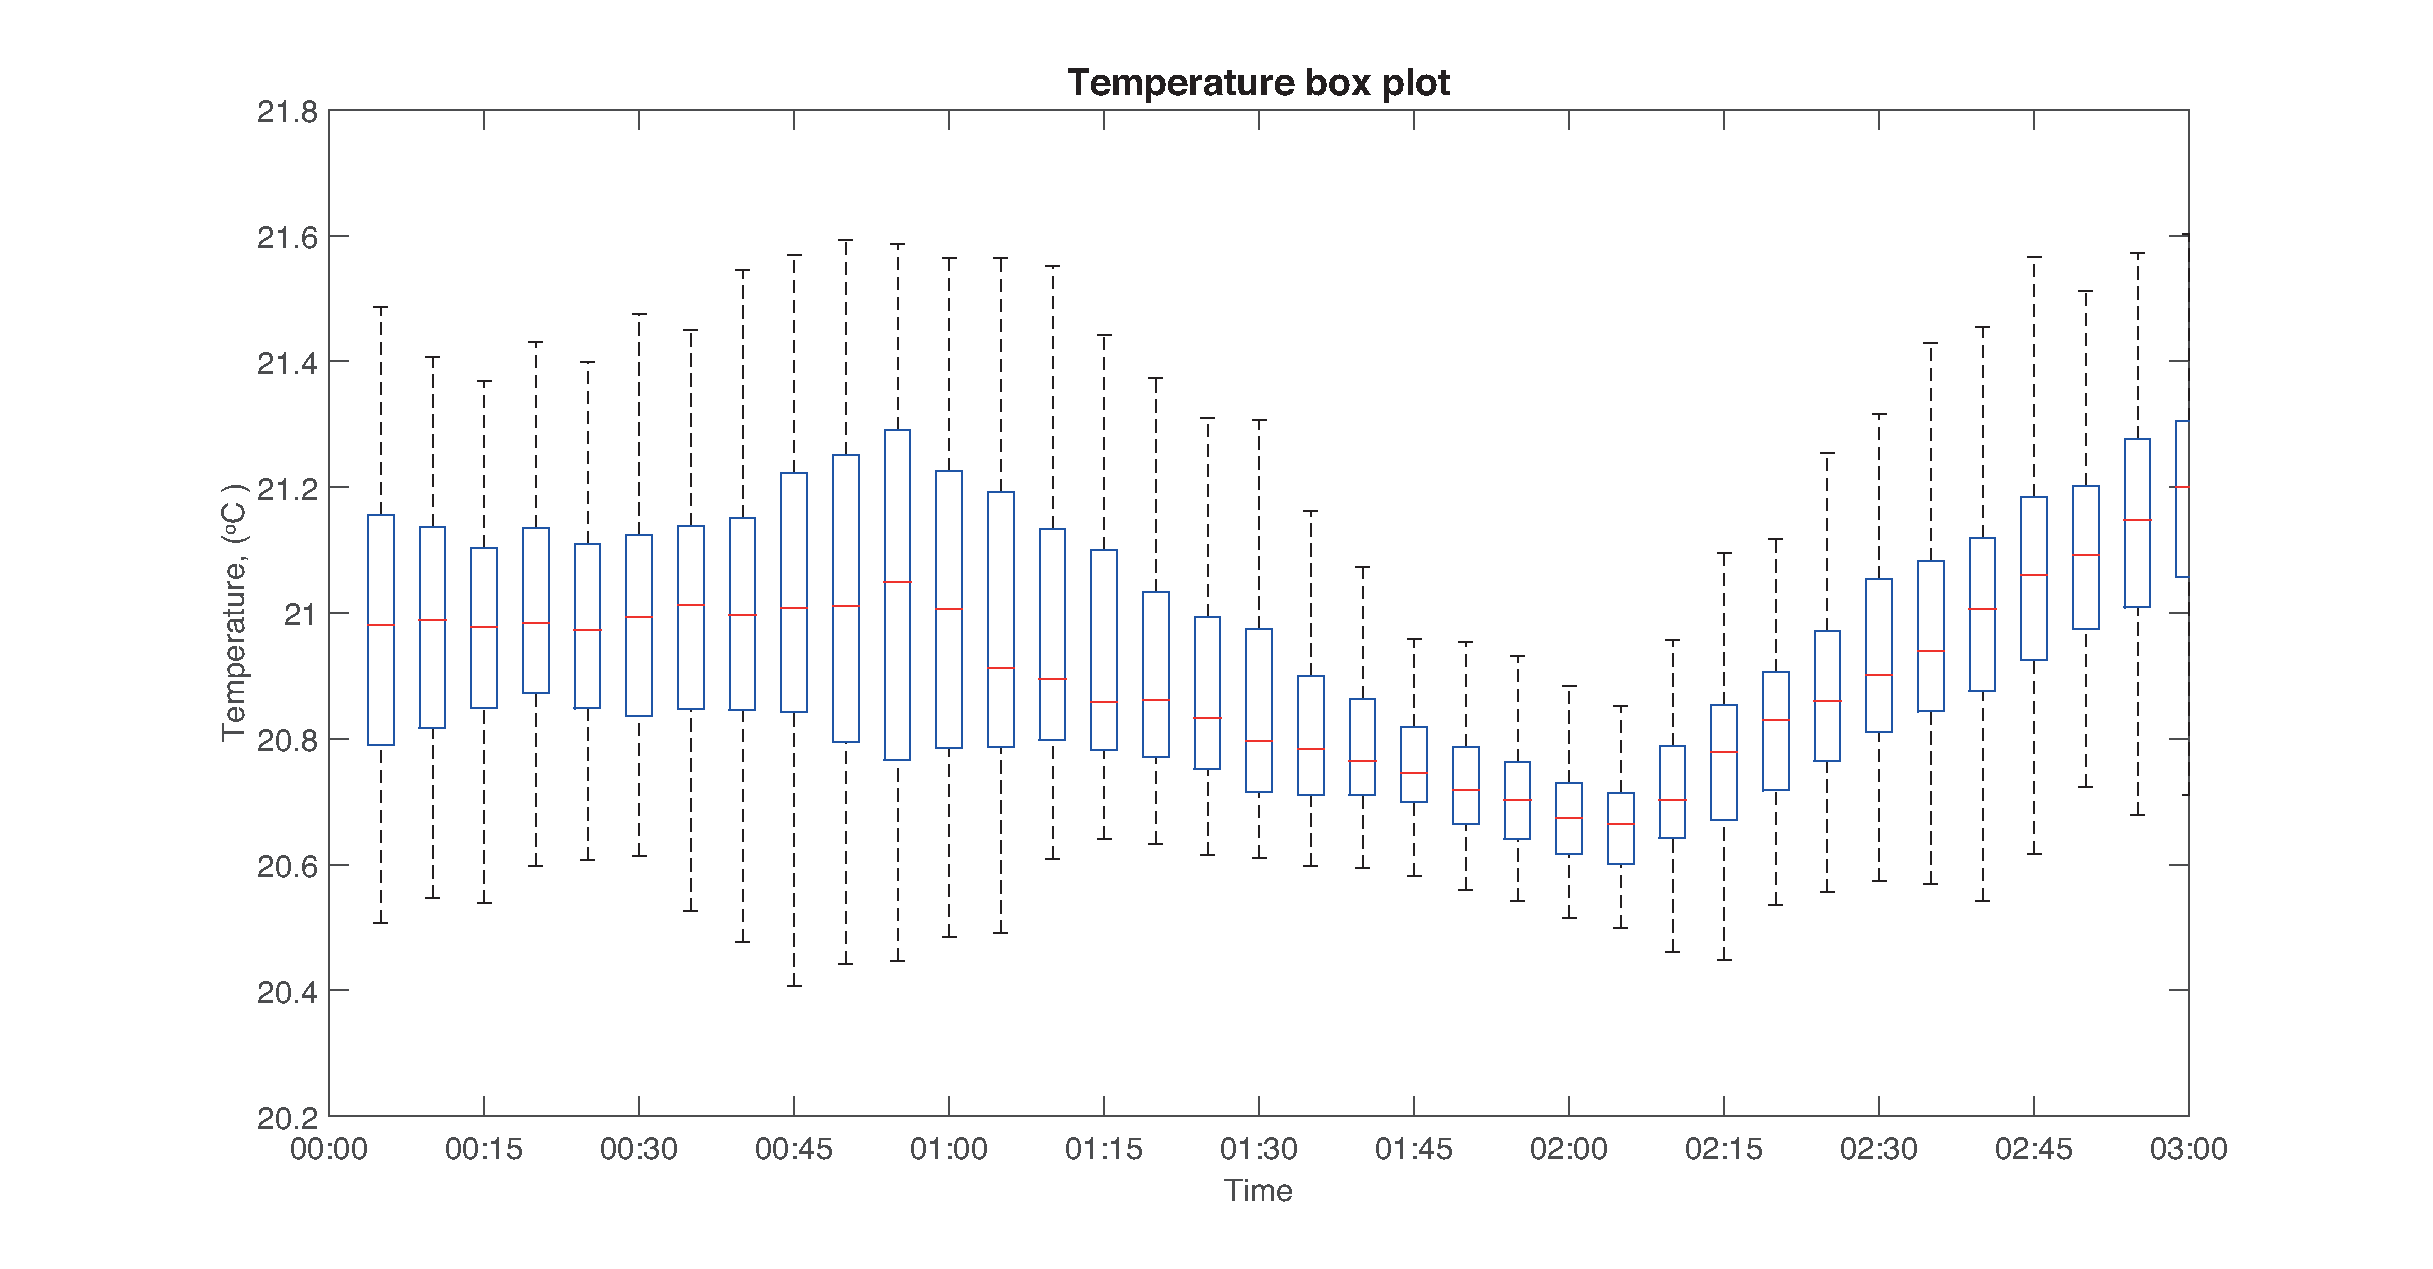
\includegraphics[width=\columnwidth]{graphics/pscc2016/agg_box_plot_100SH_0STATIC_05PCT_REDUCTION.eps}%
\label{fig:temp100}}%}
\caption{Simulation results of the 100\% availability test for the whole portfolio.}
\label{fig:test100}
\end{figure}

\begin{figure}[!t]
%\centerline{
\centering
\subfloat[Response accuracy]{\includegraphics[width=0.85\columnwidth]{graphics/pscc2016/agg_power_ctrl_70SH_30STATIC_05PCT_REDUCTION.eps}%
\label{fig:ref70}}
%\vfill
\\
\subfloat[House Temperatures]{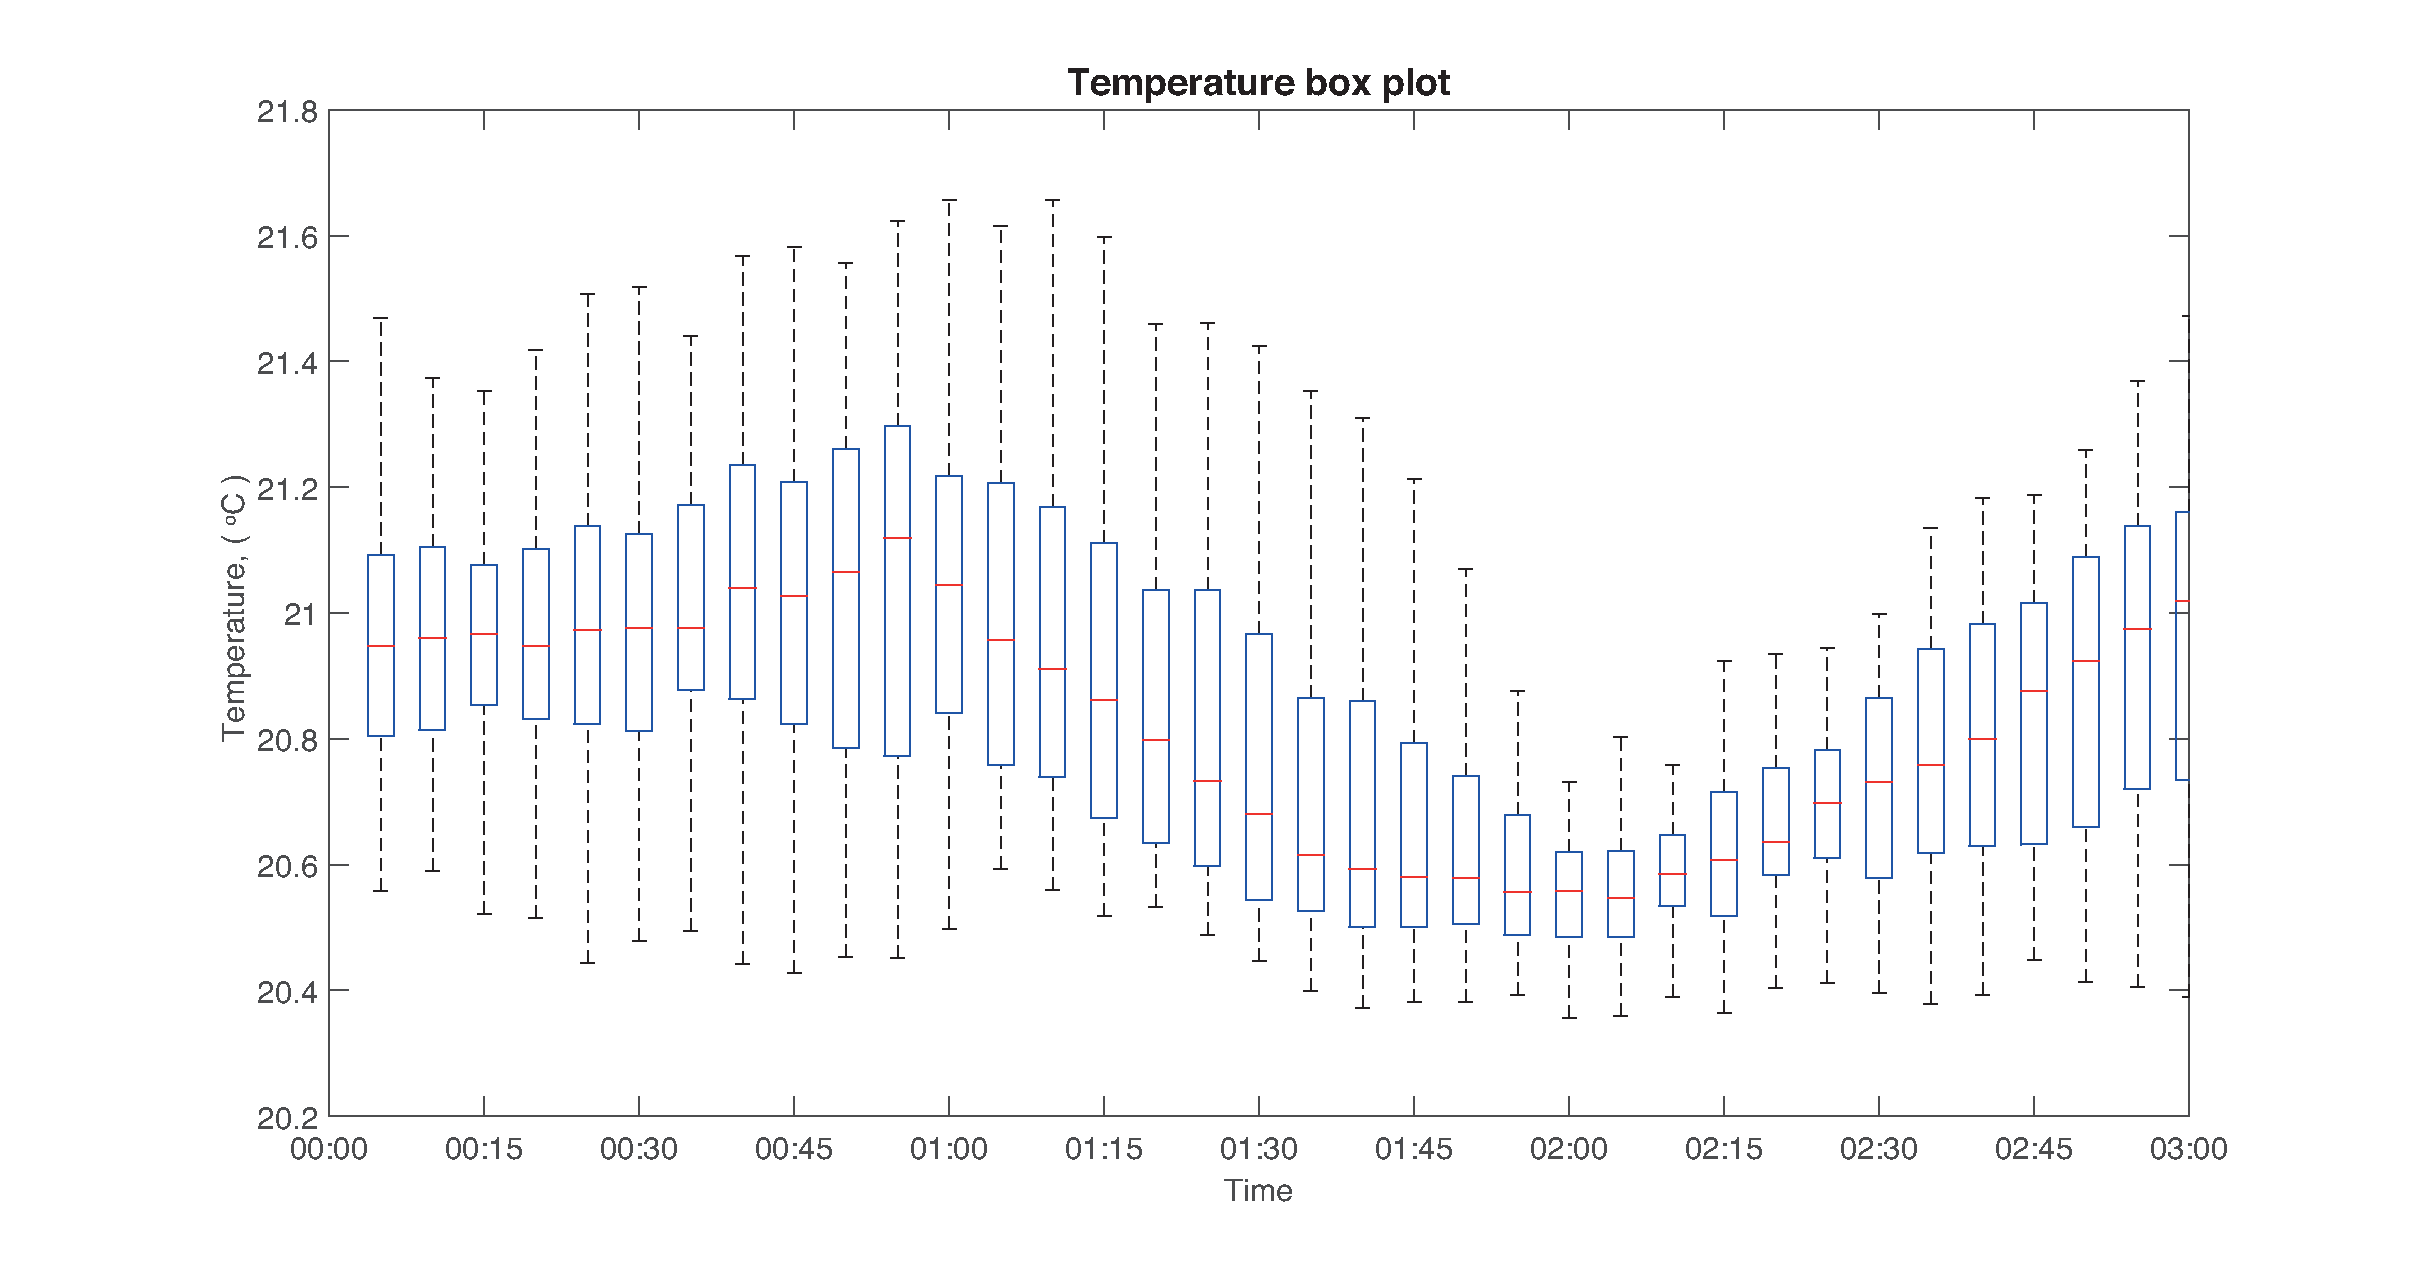
\includegraphics[width=\columnwidth]{graphics/pscc2016/agg_box_plot_70SH_30STATIC_05PCT_REDUCTION.eps}%
\label{fig:temp70}}%}
\caption{Simulation results of the 70\% availability test for the whole portfolio}
\label{fig:test70}
\end{figure}

The response accuracy of DTU-FlexServices and the average temperature of its portfolio can be seen in Fig.~\ref{fig:ref100} and Fig.~\ref{fig:ref70}. The distribution of the house temperatures can be seen in Fig.~\ref{fig:temp100} and Fig.~\ref{fig:temp70}, and it is clear that as the availability of the houses decreases, the flexibility for up-regulation is being saturated faster and the DTU-FlexServices is unable to track the FRR reference signal.

Having carried out the necessary test, RisøGrid proceeds to evaluate the results of the tests.

\subsection{Evaluation of test results}
Since the case study looks at simplified setup, and the example does not take the time responsiveness metric into account, it does not make sense to use the aggregator performance metric mentioned in Sec.~\ref{sec:evaluation}. In Sec~\ref{subsec:scenario}, the root mean square (RMS) error is chosen to measure the response accuracy metric: 
\begin{equation}
  \eta_{RMS} = \sqrt{\frac{1}{M}\sum_{i=1}^M\left(\sum_{j=1}^N\left(\Phi_{h,i,j}\right) - S_i\right)^2}
\end{equation}
where $\left[1,M\right]$ are the iterations where the aggregator has been activated. The results of the test are presented in Table~\ref{tab:results}, where it can be seen that $E[\eta_{RMS}]<60 \, kW$. Therefore the DTU-FlexServices is certified to provide FRR up-regulation service to RisøGrid.
\begingroup
\setlength{\tabcolsep}{4pt}%
\begin{table}[!t]%% increase table row spacing, adjust to taste
\renewcommand{\arraystretch}{0.9}
% if using array.sty, it might be a good idea to tweak the value of
% \extrarowheight as needed to properly center the text within the cells
\caption{Performance of DTU-FlexServices}
\label{tab:results}
\centering
% Some packages, such as MDW tools, offer better commands for making tables
% than the plain LaTeX2e tabular which is used here.
\begin{tabular}{clcccccccc}
\toprule
        & & \multicolumn{7}{c}{Process noise, $\sigma$}                   & Avg. \\
        & & 0.00   & 0.05   & 0.10   & 0.15   & 0.20   & 0.25    & 0.30   &         \\ 
\midrule
\multirow{7}{*}{\rotatebox[origin=c]{90}{Availability}} 
& 100\%   & 0.00   & 0.00   & 0.04   & 9.25   & 31.20  & 48.84   & 98.32  & 26.81   \\
& 95\%    & 0.03   & 0.00   & 1.51   & 19.19  & 37.97  & 66.56   & 102.05 & 32.47   \\
& 90\%    & 1.40   & 0.04   & 14.36  & 30.78  & 58.74  & 73.38   & 98.24  & 39.56   \\
& 85\%    & 1.10   & 35.23  & 4.06   & 45.28  & 83.06  & 83.40   & 115.11 & 52.46   \\
& 80\%    & 13.88  & 29.25  & 12.94  & 65.93  & 72.31  & 94.50   & 135.85 & 60.67   \\
& 75\%    & 54.28  & 40.74  & 39.91  & 75.22  & 86.14  & 114.13  & 135.76 & 78.03   \\
& 70\%    & 45.63  & 90.90  & 85.41  & 99.02  & 93.68  & 123.82  & 142.64 & 97.30   \\
\midrule
Avg. & & 16.62  & 28.02  & 22.60  & 49.24  & 66.16  & 86.38   & 118.28 & 55.33   \\
\bottomrule
\end{tabular}
\end{table}
\endgroup
%\begin{figure}[!t]
%\centering
%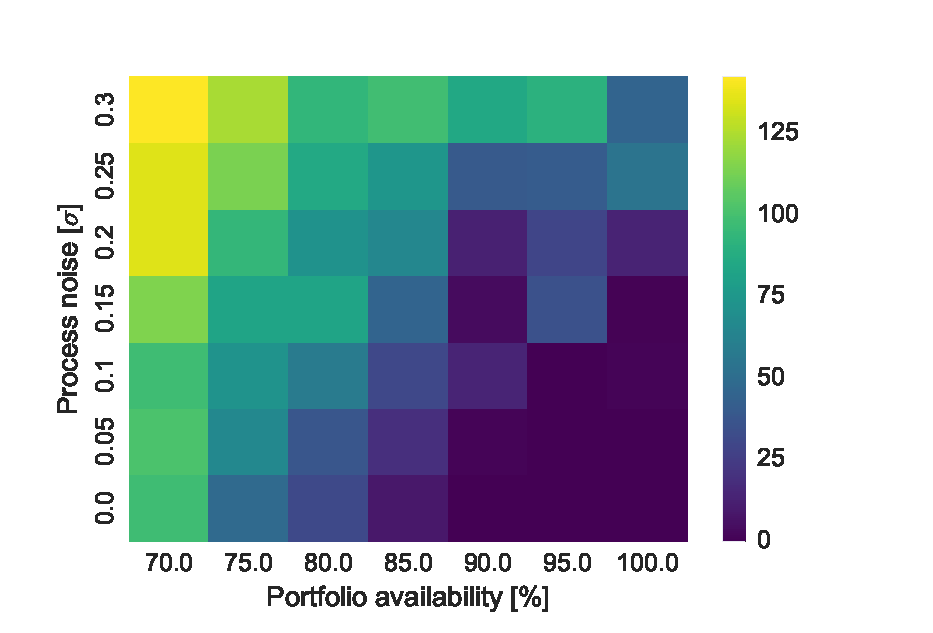
\includegraphics[width=\columnwidth]{figures/heatmap.eps}
%\caption{The RMS value over the test space. It can be seen that it is more important to have certainty in the portfolio availability than in the process noise.}
%\label{fig:colormap}
%\end{figure}

%\section{Quality Metrics}

What aspects of the aggregator influence in the performance metrics?

Internal vs. external metrics: external can be used for monitoring, internal can only manipulated in test environment.

Are there more metrics than in the table? E.g. robustness toward grid faults

\begin{table}[!t]%% increase table row spacing, adjust to taste
\renewcommand{\arraystretch}{1.3}
% if using array.sty, it might be a good idea to tweak the value of
% \extrarowheight as needed to properly center the text within the cells
\caption{System interactions can be evaluated with generalized metrics}
\label{tab:metrics}
\centering
% Some packages, such as MDW tools, offer better commands for making tables
% than the plain LaTeX2e tabular which is used here.
\begin{tabular}{ll}
\toprule
System interaction & metrics\\
\midrule
Aggregator - power system & responsiveness w.r.t. grid conditions\\
\\
Aggregator - DER portfolio & responsiveness w.r.t. time\\
 & robustness w.r.t. forecast errors\\
 \\
Aggregator -  ICT infrastructure & robustness w.r.t. communication faults\\
\bottomrule
\end{tabular}
\end{table}

\begin{table}[!t]
\renewcommand{\arraystretch}{1.3}
\caption{The quality metrics can be separated into two categories.}
\label{tab:metricsclass}
\centering
\begin{tabular}{ll}
\toprule
External metrics & Internal metrics\\
\midrule
responsiveness w.r.t. grid &robustness w.r.t. forecast errors\\
responsiveness w.r.t. time & robustness w.r.t. communication errors\\
& robustness w.r.t. grid errors\\
\bottomrule
\end{tabular}
\end{table}
\section{Conclusion and Future Work}
This work presents an initial approach to establishing a methodology for designing aggregator validation tests. This method differs from the traditional generator certification tests in that it must be carried out in simulations, so that the stochasticity of the real world disturbances affecting the aggregator can be taken into account. A drawback of this method is that it relies on the accuracy and complexity of the simulation models. This means that the components of the validation tests must be validated against reality. The test method was shown through a simplified case study on an existing aggregator. While the example shows a fictive TSO applying the test to a fictive aggregator, there is the possibility that validation of aggregators in the future will be carried out by third party test companies. 

There are still several open issues that need to be investigated with regards to aggregator validation. For example, the definition of the operation scenarios was only briefly discussed, and heuristics must be developed in order to define scenarios that are effective when testing aggregators.

An important step for the development of the validation method is the implementation of a complete test architecture with validated component models. With such a simulation framework, with realistic communication and DER models, communication delays can be implemented in order to test aggregators for time responsiveness. 

Finally, the method should be expanded to cover other ancillary services, such as voltage regulation.

We consider the work presented here an important element of enabling aggregators in the smart grid, thus enabling consumption to actively participate in the secure operation of the power system. This will help the integration of renewable energy sources into the power system.


